% Options for packages loaded elsewhere
% Options for packages loaded elsewhere
\PassOptionsToPackage{unicode}{hyperref}
\PassOptionsToPackage{hyphens}{url}
\PassOptionsToPackage{dvipsnames,svgnames,x11names}{xcolor}
%
\documentclass[
  letterpaper,
  DIV=11,
  numbers=noendperiod]{scrartcl}
\usepackage{xcolor}
\usepackage{amsmath,amssymb}
\setcounter{secnumdepth}{-\maxdimen} % remove section numbering
\usepackage{iftex}
\ifPDFTeX
  \usepackage[T1]{fontenc}
  \usepackage[utf8]{inputenc}
  \usepackage{textcomp} % provide euro and other symbols
\else % if luatex or xetex
  \usepackage{unicode-math} % this also loads fontspec
  \defaultfontfeatures{Scale=MatchLowercase}
  \defaultfontfeatures[\rmfamily]{Ligatures=TeX,Scale=1}
\fi
\usepackage{lmodern}
\ifPDFTeX\else
  % xetex/luatex font selection
\fi
% Use upquote if available, for straight quotes in verbatim environments
\IfFileExists{upquote.sty}{\usepackage{upquote}}{}
\IfFileExists{microtype.sty}{% use microtype if available
  \usepackage[]{microtype}
  \UseMicrotypeSet[protrusion]{basicmath} % disable protrusion for tt fonts
}{}
\makeatletter
\@ifundefined{KOMAClassName}{% if non-KOMA class
  \IfFileExists{parskip.sty}{%
    \usepackage{parskip}
  }{% else
    \setlength{\parindent}{0pt}
    \setlength{\parskip}{6pt plus 2pt minus 1pt}}
}{% if KOMA class
  \KOMAoptions{parskip=half}}
\makeatother
% Make \paragraph and \subparagraph free-standing
\makeatletter
\ifx\paragraph\undefined\else
  \let\oldparagraph\paragraph
  \renewcommand{\paragraph}{
    \@ifstar
      \xxxParagraphStar
      \xxxParagraphNoStar
  }
  \newcommand{\xxxParagraphStar}[1]{\oldparagraph*{#1}\mbox{}}
  \newcommand{\xxxParagraphNoStar}[1]{\oldparagraph{#1}\mbox{}}
\fi
\ifx\subparagraph\undefined\else
  \let\oldsubparagraph\subparagraph
  \renewcommand{\subparagraph}{
    \@ifstar
      \xxxSubParagraphStar
      \xxxSubParagraphNoStar
  }
  \newcommand{\xxxSubParagraphStar}[1]{\oldsubparagraph*{#1}\mbox{}}
  \newcommand{\xxxSubParagraphNoStar}[1]{\oldsubparagraph{#1}\mbox{}}
\fi
\makeatother


\usepackage{longtable,booktabs,array}
\usepackage{calc} % for calculating minipage widths
% Correct order of tables after \paragraph or \subparagraph
\usepackage{etoolbox}
\makeatletter
\patchcmd\longtable{\par}{\if@noskipsec\mbox{}\fi\par}{}{}
\makeatother
% Allow footnotes in longtable head/foot
\IfFileExists{footnotehyper.sty}{\usepackage{footnotehyper}}{\usepackage{footnote}}
\makesavenoteenv{longtable}
\usepackage{graphicx}
\makeatletter
\newsavebox\pandoc@box
\newcommand*\pandocbounded[1]{% scales image to fit in text height/width
  \sbox\pandoc@box{#1}%
  \Gscale@div\@tempa{\textheight}{\dimexpr\ht\pandoc@box+\dp\pandoc@box\relax}%
  \Gscale@div\@tempb{\linewidth}{\wd\pandoc@box}%
  \ifdim\@tempb\p@<\@tempa\p@\let\@tempa\@tempb\fi% select the smaller of both
  \ifdim\@tempa\p@<\p@\scalebox{\@tempa}{\usebox\pandoc@box}%
  \else\usebox{\pandoc@box}%
  \fi%
}
% Set default figure placement to htbp
\def\fps@figure{htbp}
\makeatother





\setlength{\emergencystretch}{3em} % prevent overfull lines

\providecommand{\tightlist}{%
  \setlength{\itemsep}{0pt}\setlength{\parskip}{0pt}}



 


\KOMAoption{captions}{tableheading}
\makeatletter
\@ifpackageloaded{caption}{}{\usepackage{caption}}
\AtBeginDocument{%
\ifdefined\contentsname
  \renewcommand*\contentsname{Table of contents}
\else
  \newcommand\contentsname{Table of contents}
\fi
\ifdefined\listfigurename
  \renewcommand*\listfigurename{List of Figures}
\else
  \newcommand\listfigurename{List of Figures}
\fi
\ifdefined\listtablename
  \renewcommand*\listtablename{List of Tables}
\else
  \newcommand\listtablename{List of Tables}
\fi
\ifdefined\figurename
  \renewcommand*\figurename{Figure}
\else
  \newcommand\figurename{Figure}
\fi
\ifdefined\tablename
  \renewcommand*\tablename{Table}
\else
  \newcommand\tablename{Table}
\fi
}
\@ifpackageloaded{float}{}{\usepackage{float}}
\floatstyle{ruled}
\@ifundefined{c@chapter}{\newfloat{codelisting}{h}{lop}}{\newfloat{codelisting}{h}{lop}[chapter]}
\floatname{codelisting}{Listing}
\newcommand*\listoflistings{\listof{codelisting}{List of Listings}}
\usepackage{amsthm}
\theoremstyle{definition}
\newtheorem{example}{Example}[section]
\theoremstyle{remark}
\AtBeginDocument{\renewcommand*{\proofname}{Proof}}
\newtheorem*{remark}{Remark}
\newtheorem*{solution}{Solution}
\newtheorem{refremark}{Remark}[section]
\newtheorem{refsolution}{Solution}[section]
\makeatother
\makeatletter
\makeatother
\makeatletter
\@ifpackageloaded{caption}{}{\usepackage{caption}}
\@ifpackageloaded{subcaption}{}{\usepackage{subcaption}}
\makeatother
\usepackage{bookmark}
\IfFileExists{xurl.sty}{\usepackage{xurl}}{} % add URL line breaks if available
\urlstyle{same}
\hypersetup{
  pdftitle={Simulation Challenge},
  colorlinks=true,
  linkcolor={blue},
  filecolor={Maroon},
  citecolor={Blue},
  urlcolor={Blue},
  pdfcreator={LaTeX via pandoc}}


\title{Simulation Challenge}
\usepackage{etoolbox}
\makeatletter
\providecommand{\subtitle}[1]{% add subtitle to \maketitle
  \apptocmd{\@title}{\par {\large #1 \par}}{}{}
}
\makeatother
\subtitle{Generative Models and Monte Carlo Simulation}
\author{}
\date{}
\begin{document}
\maketitle


\section{🎲 Simulation Challenge - Monte Carlo
Analysis}\label{simulation-challenge---monte-carlo-analysis}

\subsection{Challenge Overview}\label{challenge-overview}

\textbf{Your Mission:} Create a comprehensive Quarto document that
simulates one or two investment strategies, analyzes the results, and
demonstrates your ability to present counter-intuitive findings
compellingly. Then render the document to HTML and deploy it via GitHub
Pages from a new repository called ``simulationChallenge.''

\subsection{The Investment Game 🎯}\label{the-investment-game}

\subsubsection{Original Game Strategy}\label{original-game-strategy}

\begin{example}[]\protect\hypertarget{exm-ErgodicityEconomicsExample}{}\label{exm-ErgodicityEconomicsExample}

Imagine you are offered the following game and given a \$1,000 budget in
a special account to play the game: I will flip a coin, and if it comes
up heads, we increase your account's balance by 50\%; if it comes up
tails, we reduce your account's balance by 40\%. We are not only doing
this once, but we will do it once per year until you turn 55. When you
turn 55, you will receive the balance in your account.

\end{example}

\subsubsection{Generative DAG Model for the Investment
Game}\label{generative-dag-model-for-the-investment-game}

\subsection{Challenge Requirements 📋}\label{challenge-requirements}

\subsubsection{Questions to Answer for 75\% Grade on
Challenge}\label{questions-to-answer-for-75-grade-on-challenge}

\begin{enumerate}
\def\labelenumi{\arabic{enumi}.}
\item
  \textbf{Expected Value Analysis:} What is the ``expected value'' of
  your account balance after 1 coin flip for the original game?
\item
  \textbf{Expectation vs.~Reality:} Is the expected value positive or
  negative? Do you expect your account to be worth more or less than
  \$1,000 based on this result?
\item
  \textbf{Single Simulation:} Run one simulation showing the dynamics of
  your account balance over time. Make an object-oriented matplotlib OR
  ggplot2 plot showing your simulated account balance over time (i.e.~as
  you age). Comment on the results, are you happy?
\end{enumerate}

\subsection{Analysis and Solutions}\label{analysis-and-solutions}

\subsubsection{Question 1: Expected Value
Analysis}\label{question-1-expected-value-analysis}

\textbf{What is the ``expected value'' of your account balance after 1
coin flip for the original game?}

Let's calculate this step by step using R:

\begin{verbatim}
Expected Value Calculation:
\end{verbatim}

\begin{verbatim}
========================
\end{verbatim}

\begin{verbatim}
Initial Balance: $ 1000 
\end{verbatim}

\begin{verbatim}
Heads (50% chance): $ 1000  × 1.5 = $ 1500 
\end{verbatim}

\begin{verbatim}
Tails (50% chance): $ 1000  × 0.6 = $ 600 
\end{verbatim}

\begin{verbatim}

Expected Value = 0.5 × $ 1500  + 0.5 × $ 600 
\end{verbatim}

\begin{verbatim}
Expected Value = $ 750  + $ 300 
\end{verbatim}

\begin{verbatim}
Expected Value = $ 1050 
\end{verbatim}

\begin{verbatim}

Simulation Verification:
\end{verbatim}

\begin{verbatim}
=======================
\end{verbatim}

\begin{verbatim}
Simulated Expected Value (10,000 trials): $ 1044.87 
\end{verbatim}

\begin{verbatim}
Theoretical Expected Value: $ 1050 
\end{verbatim}

\begin{verbatim}
Difference: $ 5.13 
\end{verbatim}

\subsubsection{Question 2: Expectation
vs.~Reality}\label{question-2-expectation-vs.-reality}

\textbf{Is the expected value positive or negative? Do you expect your
account to be worth more or less than \$1,000 based on this result?}

\begin{verbatim}
Expectation vs. Reality Analysis:
\end{verbatim}

\begin{verbatim}
================================
\end{verbatim}

\begin{verbatim}
Initial Investment: $ 1000 
\end{verbatim}

\begin{verbatim}
Expected Value after 1 flip: $ 1050 
\end{verbatim}

\begin{verbatim}
Expected Gain/Loss: $ 50 
\end{verbatim}

\begin{verbatim}
Expected Return:  5 %
\end{verbatim}

\begin{verbatim}

✅ The expected value is POSITIVE!
Based on this result, I expect my account to be worth MORE than $1,000.
This suggests the game is favorable in the long run.
\end{verbatim}

\begin{verbatim}

🤔 But wait! Let's think about this more carefully...
\end{verbatim}

\begin{verbatim}
The expected value calculation assumes we can play this game many times.
\end{verbatim}

\begin{verbatim}
But in reality, we only get to play once per year until age 55.
\end{verbatim}

\begin{verbatim}
This is a key insight about ergodicity economics!
\end{verbatim}

\subsubsection{Question 3: Single
Simulation}\label{question-3-single-simulation}

\textbf{Run one simulation showing the dynamics of your account balance
over time. Make an object-oriented ggplot2 plot showing your simulated
account balance over time (i.e.~as you age). Comment on the results, are
you happy?}

Let's simulate the investment game over multiple years to see how the
account balance evolves:

\begin{verbatim}
Single Investment Simulation Results:
\end{verbatim}

\begin{verbatim}
====================================
\end{verbatim}

\begin{verbatim}
Starting Age: 25
\end{verbatim}

\begin{verbatim}
Ending Age: 55
\end{verbatim}

\begin{verbatim}
Initial Balance: $ 1000 
\end{verbatim}

\begin{verbatim}
Final Balance: $ 205.89 
\end{verbatim}

\begin{verbatim}
Total Return:  -79.4 %
\end{verbatim}

\begin{verbatim}
Annualized Return:  -5.1 %
\end{verbatim}

\begin{verbatim}

First 5 years:
\end{verbatim}

\begin{verbatim}
# A tibble: 6 x 2
    age balance
  <dbl>   <dbl>
1    25    1000
2    26     600
3    27     360
4    28     540
5    29     810
6    30    1215
\end{verbatim}

\begin{verbatim}

Last 5 years:
\end{verbatim}

\begin{verbatim}
# A tibble: 5 x 2
    age balance
  <dbl>   <dbl>
1    51    254.
2    52    381.
3    53    572.
4    54    343.
5    55    206.
\end{verbatim}

\begin{figure}[H]

{\centering \pandocbounded{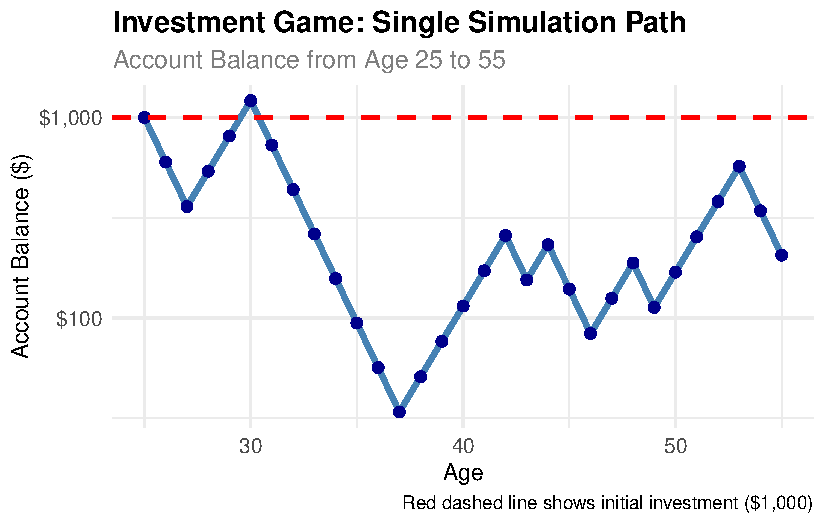
\includegraphics[keepaspectratio]{index_files/figure-pdf/single-simulation-1.pdf}}

}

\caption{Single simulation of investment game showing account balance
over time}

\end{figure}%

\begin{verbatim}

📊 Analysis of Single Simulation:
\end{verbatim}

\begin{verbatim}
================================
\end{verbatim}

\begin{verbatim}
❌ This simulation was UNSUCCESSFUL!
The account shrank from $ 1000  to $ 205.89 
This represents a loss of $ 794.11 
\end{verbatim}

\begin{verbatim}

Year-by-year breakdown:
\end{verbatim}

\begin{verbatim}
Winning years:  15 
\end{verbatim}

\begin{verbatim}
Losing years:  15 
\end{verbatim}

\begin{verbatim}
Win rate:  50 %
\end{verbatim}

\begin{verbatim}

🤔 Key Insights:
\end{verbatim}

\begin{verbatim}
===============
\end{verbatim}

\begin{verbatim}
1. Despite a positive expected value (+5% per year), this single path shows the reality of randomness.
\end{verbatim}

\begin{verbatim}
2. The multiplicative nature of the game means early losses are very hard to recover from.
\end{verbatim}

\begin{verbatim}
3. This single simulation doesn't tell us the full story - we need to look at many simulations.
\end{verbatim}

\begin{verbatim}
4. The log scale plot shows the exponential nature of the growth/decay process.
\end{verbatim}




\end{document}
